\chapter{\label{chap:2grundlagen}Grundlagen der Blockchain-Technologie}

Allgemein lässt sich eine Blockchain als geordnete, rückverkettete Liste von Blöcken, also als eine verteilte Datenstruktur\cite{Block}, in der digitale Datensätze, Ereignisse oder Transaktionen gespeichert werden, bechreiben. 
Durch die Verwendung von Kryptohash-Werten und asymmetrischer Verschlüsselung wird die Fälschungssicherheit der Blockchain gewährleistet. Ein dezentralisiertes Peer-to-Peer Netzwerk verteilt die Blockchain auf eine Vielzahl von Knotenpunkten, um die Verfügbarkeit und Ausfallsicherheit zu erhöhen\cite{bafin}. 

	\section{Kryptographische Hashfunktionen}
		
		Hash- oder Streuwertfunktionen sind Funktionen, die eine beliebig große Eingabemenge auf eine kleinere Ausgabemenge abbilden. Die Länge der Eingabe spielt hierbei keine Rollen, wobei die Länge der Ausgaben immer gleich sein sollte. Hashfunktionen sind deterministisch, das heißt bei gleicher Eingabe muss auch das gleiche Ergebnis erzielt werden. Diese Berechnung der Hash-Werte soll möglichst schnell von statten gehen. Für einige Anwednungsfälle ist ein zusätzliches Kriterium, dass wenn sich ein Zeichen des Eingabewertes ändert, sich möglichst viele des Stellen des Zielwertes ändern sollen. Ein Rückschluss von Hash- auf Eingabewert soll nicht effektiv möglich sein, was man als "`Einwegfunktion"' bezeichnet \cite{kh}.
		
		Die bisher genannten Eigenschaften sollten sowohl auf Hashfunktionen als auch Kryptologische Hashfunktionen zutreffen. Bedingungen, die für eine Kryptologische Hashfunktion aber für eine normale Hashfunktion nicht zwingend erfüllt sein müssen, sind die schwache und starke Kollisionsresistenz. Schwache Kollisionsresistenz bedeutet, dass es nicht effektiv möglich sein darf zu einem gegebenen Eingabewert einen weiteren Wert zu finden, sodass deren beide Ergebnishashes gleich sind. Starke Kollisionsresistenz bedeutet, dass es nicht effektiv möglich sein darf überhaupt ein solches Paar aus der gesamten möglichen Eingabemenge zu finden, deren Ergebnishashes gleich sind. Einige Kryptologische Hashfunktionen haben zusätzlich die Möglichkeit einen zusätzlichen Schlüssel für die Funktion anzugeben, sodass beispielswesie zwei Werte mit unterschiedlichem Schlüssel auch unterschiedliche Hashes erzeugen. Diese Eigenschaft ist allerdings kein zwingendes Kriterium für eine Kryptologische Hashfunktion. Die 4 Kernanforderungen für Kryptologische Hashes werden in der folgenden Liste dargestellt: 
		\newpage
		
\begin{enumerate}
\item{Effiziente / Schnelle Berechnung}
\item{Einwegfunktion}
\item{Schwache Kollisionsresistenz}
\item{Starke Kolissionsresistenz}
\end{enumerate}
		
		Aufgrund der immer größer werdenden Rechenleistungen von Computern und beispielsweise dafür eingesetzen Großrechnern oder Computer-Cluster gibt es weite Diskussionen darüber, welche (Kryptolgischen) Hashfunktionen tatsächlich (noch) sicher sind. Die am weitesten verbreiteten Kryptologischen Hashfunktionen sind die SHA-"'X"' und MD"'X"' Reihen, wobei "`X"' für den jeweiligen Versionsname steht \cite{shamd}. Auch bei diesen Hash-Familien wird mittlerweile von der Verwendung alter Versionen aufgrund mangelnder Sicherheit abgeraten. Bei den aktuellen Vertretern dieser Hashes geht man aber von ausreichender Sicherheit aus.
		
	\section{\label{subsec:p2p}Dezentralisierte Netzwerkstrukturen}
	
		Ein Grundprinzip der Blockchain ist das Peer-to-Peer Netzwerk. Teilnehmer des Netzwerkes werden Knoten oder Peer genannt. In Abbildung \ref{net} ist ein zentralisiertes Netzwerk zu sehen. Alle Knoten sind über eine zentrale Komponente mit einander verbunden. Der gesamte Netzwerkverkehr liegt auf seiten der zentralen Verbindungskomponente. Desweiteren ist eine Kommunikation im Netz bei Ausfall der zentralen Komponente nicht mehr gewährleistet. 
Die Blockchain verwendet ein verteiltes bzw. vermaschtes Netzwerk. Dieses ist in Abbildung \ref{net} dargestellt. In diesem Netzwerk existiert keine zentrale Komponente. Viel mehr entstehen durch Verbindungen zu mehreren Knoten Redundanzen im Netzwerk. Solange der gegenüberliegende Knoten aktiv ist, kann mit ihm kommuniziert werden, ohne dass die Daten auf einem Server oder einer anderen zentralen Stelle zwischengespeichert werden müssen. Falls einer der Knoten ausfällt, gibt es noch weitere Knoten, auf die zurückgegriffen werden kann. In der Regel werden mehrere Verbindungen aufrecht erhalten, um die Redundanz zu gewährleisten. 
		
    \begin{figure}[htbp]
    \subfigure[Zentralisiertes Netz \cite{star}]{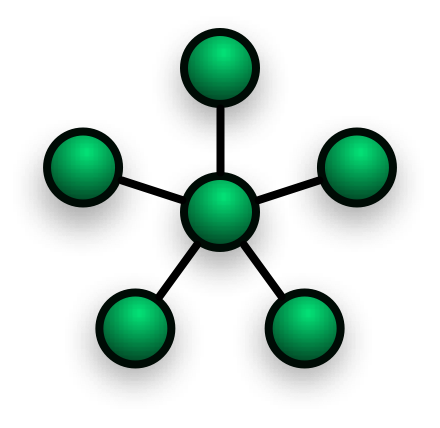
\includegraphics[width=0.49\textwidth]{Bilder/star.png}} 
    \subfigure[Verteiltes Netz \cite{mesh}]{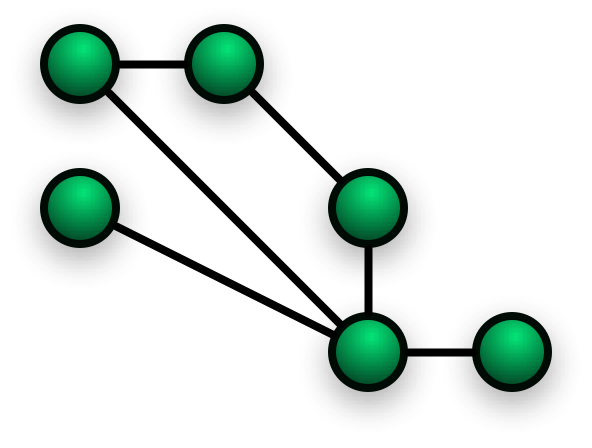
\includegraphics[width=0.49\textwidth]{Bilder/mesh.png}} 
    \caption{Netztopologien} 
    \label{net}
    \end{figure}
		
		Die Blockchain wird über ein Peer-to-Peer Netzwerk auf die einzelnen Konten verteilt. Transaktionen innerhalb des Netzwerkes werden als neuer Zustand in der Blockchain gespeichert. Jeder Knoten des Netzwerkes hält eine Kopie der Blockchain. \\
		Der Begriff der Dezentralisierung bekommt bei der Blockchain eine besondere Bedeutung. Die Dezentralisierung des Netzwerkes sorgt nicht nur für Ausfallsicherheit, sondern auch für Unabhängigkeit. So ist es praktisch unmöglich für einen einzelnen die Informationen, die in der Blockchain gespeichert sind zu verändern oder zu zensieren.
		
	
	\section{Asymmetrische Kryptographie}
		
Um an einem auf Blockchain basierenden System teilzunehmen, braucht es eine Zugangssoftware. Die Zugangssoftware wird als Wallet bezeichnet und besteht aus einem öffentlichen und privaten Schlüssel. Die aus der asymmetrischen Verschlüsselung stammende Technik wird zur Signierung und Adressierung der kryptografischen Währung genutzt \cite{stallings}. Zu den bekanntesten asymmetrischen Verschlüsselungsverfahren zählen RSA und Diffie-Hellman \cite{RSADH}.
Der öffentliche Schlüssel dient als Adresse der Wallet, vergleichbar mit der IBAN-Nummer eines Kontos. Außerdem kann mit Hilfe des öffentlichen Schlüssels, der Kontostand einer Wallet eingesehen werden. Jedoch dient der öffentliche Schlüssel als Pseudonym, so dass es nicht möglich ist, aus ihm die Identität des Besitzers zu ermitteln. Dieser öffentliche Schlüssel wird bekannt gegeben. Für Transaktionen benötigt man den eigenen privaten Schlüssel, welcher als Pin der eigenen Wallet fungiert \cite{priv}. Der Absender kombiniert die Nachricht mit seinem privaten Schlüssel und sendet die signierte Nachricht an die sich aus dem öffentlichen Schlüssel ergebende Adresse des Empfängers. Mit dem öffentlichen Schlüssel des Absenders kann der Empfänger die signierte Nachricht prüfen und somit die Authentizität der Nachricht verifizieren \cite{badev}. Der Absender der Nachricht kann nicht leugnen, diese signiert zu haben \cite{franco}. Durch die assymmetrische Verschlüsselung kann die Nachricht nicht unbemerkt verändert werden, wodurch deren Integrität gewährleistet ist \cite{stallings}.
	
	\section{Kryptowährungen}
	
		Kryptografische Währungen sind eine Art digitales Geld. Im Internet sind diese vielseitig einsetzbar. Zu den größten kryptografischen Währungen zählen Bitcoin und Ethereum. Mit ihnen können online Einkäufe getätigt oder weltweit innerhalb von kürzester Zeit digitale Währungsbeträge versendet werden. Außerdem werden sie wie die üblichen Währungen auf dem Währungsmarkt gehandelt und Investoren nutzen sie als Geldanlage genutzt.\\
		Der wesentliche Unterschied zwischen gewöhnlichem Geld und Kryptowährungen ist die Regulierung sowie die Entstehung des Geldes. Normales Geld wird von einer Zentralbank herausgegeben. Im Vergleich dazu entstehen kryptografische Währungen durch Blockchain-Prozesse. \\
		Kryptowährungen existieren bis auf wenige Ausnahmen (IOTA) nur in der Blockchain. Durch eine Wallet erhält der Besitzer Zugriff auf seine im Besitz befindlichen Währungsanlagen.\\
		Da Digitalwährungen nur in der Blockchain existieren, gibt es sie auch nicht in Form von Bargeld im klassischen Sinne. Von einigen Währungen, beispielsweise Bitcoin, können jedoch auch echte Münzen erworben werden, die den geheimen Code eines einzelnen Bitcoins beinhalten. Allerdings ist hierbei besondere Vorsicht geboten, denn solange der Code noch nicht in die Wallet des Erwerbers übertragen wurde, ist er anfällig für Angriffe und kann sogar von dem Verkäufer der Münze \glqq{}zurückgeklaut\grqq{} werden, falls dieser den Code noch kennt. \cite{kcur}	
		
	\subsection{Bitcoin}\label{subsec:bitcoin}	
	
		Bitcoin war die erste Kryptowährung und ist maßgeblich dafür verantwortlich, dass der Begriff Blockchain heute so bekannt ist \cite{BITB}. Das Bitcoinsystem ist vollständig und gut in einem Wiki \cite{BC-Wiki} dokumentiert und wird in vielen Arbeiten behandelt oder als Beispiel genutzt. 
		Das Bitcoin-Konzept wurde ertsmals 2008 unter dem Pseudonym Satoshi Nakamoto in einem White Paper vorgeschlagen \cite{BC}. Das Einheitenzeichen für Bitcoin ist BTC, welches auch oft als Abkürzung verwendet wird. \\
		Für die Generierung von Bitcoins müssen Knoten des Peer-to-Peer Netzwerkes Lösungen zu einem bestimmten, schwer lösbaren mathematischen Problem finden. In den ersten vier Jahren seit Bestehen des Bitcoin-Netzwerkes wurden 10.500.000 Bitcoin geschaffen. Aller vier Jahre wird dieser Betrag halbiert, sodass sich über die Zeit, die Gesamtzahl an Bitcoins 21 Millionen annähern wird. Der letzte Block, welcher eine Münze generiert, wird mit dem jetzigen System etwa im Jahr 2140 erreicht werden. Die derzeitige Größe der Bitcoin-Blockchain beträgt 159 Gigabyte (Stand März 2018) \cite{BCS} . \\
		Im Bitcoinsystem wird der Konsensmechanismus Proof-of-Work verwendet. Das Ziel aller Konsensmechanismen ist es, einen Konsens zwischen gegenseitig nicht vertrauenswürdigen Teilnehmern ohne vertrauenswürdigen Dritten zu bilden \cite{Block}. Der Grundgedanke von Konsensmechanismen ist es, dass kein Teilnehmer allein den aktuellen Zustandes des Netzwerkes oder eines Teils davon bestimmen kann, es gleichzeitig aber jedem Teilnehmer potenziell möglich ist den Zustand des Netzwerkes zu verändern. Der jeweilige Konsensmechanismus gibt die Bedingungen vor, die ein Teilnehmer erfüllen muss, um den Zustand des Netzwerkes verändern zu dürfen \cite{BITB}. Im Kontext von Blockchain-Netzwerken besteht die Veränderung darin, einen Block anzuhängen. Oft wird auch von generieren, erzeugen oder minen eines Blockes gesprochen.
		Die Bedingung muss von einem einzelnen Teilnehmer nur schwer zu erbringen, von allen anderen Teilnehmern aber leicht überprüfbar sein. Dabei bezieht sich schwer oft auf hohen Rechenaufwand oder eine geringe Wahrscheinlichkeit.\\ 
		Bei Proof-of-Work ist die Bedingung der Nachweis einer gewissen Rechenleistung. Dieser Mechanismus wird von Nakamoto mit \textit{one-vote-per-cpu} beschrieben \cite{PoW, BC}.
		In Bitcoin ist dafür in jedem Block eine Zahl enthalten, die so gewählt oder besser gefunden werden muss, dass der Hashwert des Blocks kleiner als ein vom Netzwerk vorgegebener Wert ist. Für jeden Teilnehmer ist der zu berechnende Block unterschiedlich, da die erste Transaktion jedes Blockes eine Transaktion \textit{aus dem Nichts} an den Teilnehmer selbst ist und dort der individuelle öffentliche Schlüssel hinterlegt ist. Dadurch und durch die niedrige Warscheinlichkeit die richtige Zahl zu erraten, kann nicht vorhergesagt werden, welcher Teilnehmer den nächsten gültigen Block generiert \cite{PoW}.
		Proof-of-Work kann theoretisch einen Teilnehmer mit einer Rechenleistung von \(<50\%\) der Gesamtrechenleistung des Netzwerkes kompensieren. Praktisch wird das Netzwerk aber schon ab \(25\%\) instabil \cite{CC}.
		
	\subsection{Ethereum}
	
		Das Ethereum-System baut auf dem Prinzip der Blockchain auf und dient zur Handhabung von kryptografischen Währungen. Dabei wird Ether als interne Währung im Ethereum-System verwendet. Im Zusammenhang mit Ethereum sind auch Smart Contracts zu nennen. Dabei handelt es sich um Programme, welche automatisch ausgeführt werden, sobald eine festgelegte Summe Ether überwiesen wurde. Nach der Überweisung startet automatisch die im Vertrag festgelegte Dienstleistung. Smart Contracts werden in der für Ethereum entwickelten Programmiersprache Solidity geschrieben. Desweiteren können dezentralisierte Applikationen auf der Blockchain ausgeführt werden, diese werden durch Smart Contracts beschrieben. \\
		Ethereum wurde durch die Publikationen Ethereum: A Next Generation Smart Contract and Decentralized Application Platform (2013) \cite{ETHW} und Ethereum Yellow Paper (2014) \cite{ETHY} beschrieben. Zu den Entwicklern und Mitbegründern des Ethereum-Projekts gehören Vitalik Buterin, Gavin Wood und Jeffrey Wilcke. Der Betrieb des Ethereum-Netzwerkes startete Juli 2015 \cite{ETHT}. \\
		Als Konsensmechanismus wird Proof-of-Work verwendet, jedoch ist im Entwicklungsplan von Ethereum vorgesehen, dass der Mechanismus auf Proof-of-Stake verändert wird \cite{ETHE}. Proof-of-Work ist sehr rechenintensiv. Proof-of-Stake als Alternative, ist ein deutlich weniger rechenaufwendiger Mechanismus. Die Bedingung ist der Besitz von Anteilen von Token im Netzwerk. Je mehr Anteile ein Teilnehmer besitzt, desto wahrscheinlicher generiert er einen Block \cite{BITB}.
		
	\subsection{Vergleich der Exemplare}
	
		Sowohl Bitcoin als auch Ethereum nutzen die Blockchain als Grundlage ihres Netzwerkes. Bei Bitcoin handelt es sich außerdem um eine Währung, Ethereum nutzt dabei Ether als Währung im eigenen System. Bitcoin wurde im Jahr 2009 vorgestellt. Ethereum erstmals im Jahr 2013, allerdings handelt es sich bei Ethereum auch um ein Projekt, welches seit dem ständig fortentwickelt wurde. Erkennbar ist es unter anderem, dass der Konsensmechanismus bei Ethereum im Laufe der Entwicklung von Proof-of-Work zu Proof-of-Stake wird. Bitcoin nutzt seit der Vorstellung Proof-of-Work als Konsensmechanismus.\\
		Ein wesentlicher Unterschied ist die Verwendung von Smart Contracts und dezentralisierten Applikationen bei Ethereum. Dadurch wird die Nutzung des Ethereum-Netzwerkes flexibler im Vergleich zum Bitcoin-Netzwerk. 		
